\documentclass[tikz,border=12pt]{standalone}
\usepackage[T1]{fontenc}
\usepackage{mathpazo}
\usepackage{amsmath,amssymb}
\usetikzlibrary{arrows.meta, positioning, calc, fit, decorations.pathreplacing}

\definecolor{stblue}{HTML}{7B97AD}
\definecolor{rwgold}{HTML}{B8995E}
\definecolor{sage}{HTML}{7A9A7E}
\definecolor{dkbrown}{HTML}{3D3530}
\definecolor{wmgray}{HTML}{7B7067}
\definecolor{cream}{HTML}{F9F6F0}
\definecolor{border}{HTML}{D4C9B8}
\definecolor{terracotta}{HTML}{C47A6A}
\definecolor{lavender}{HTML}{907EA0}

\begin{document}
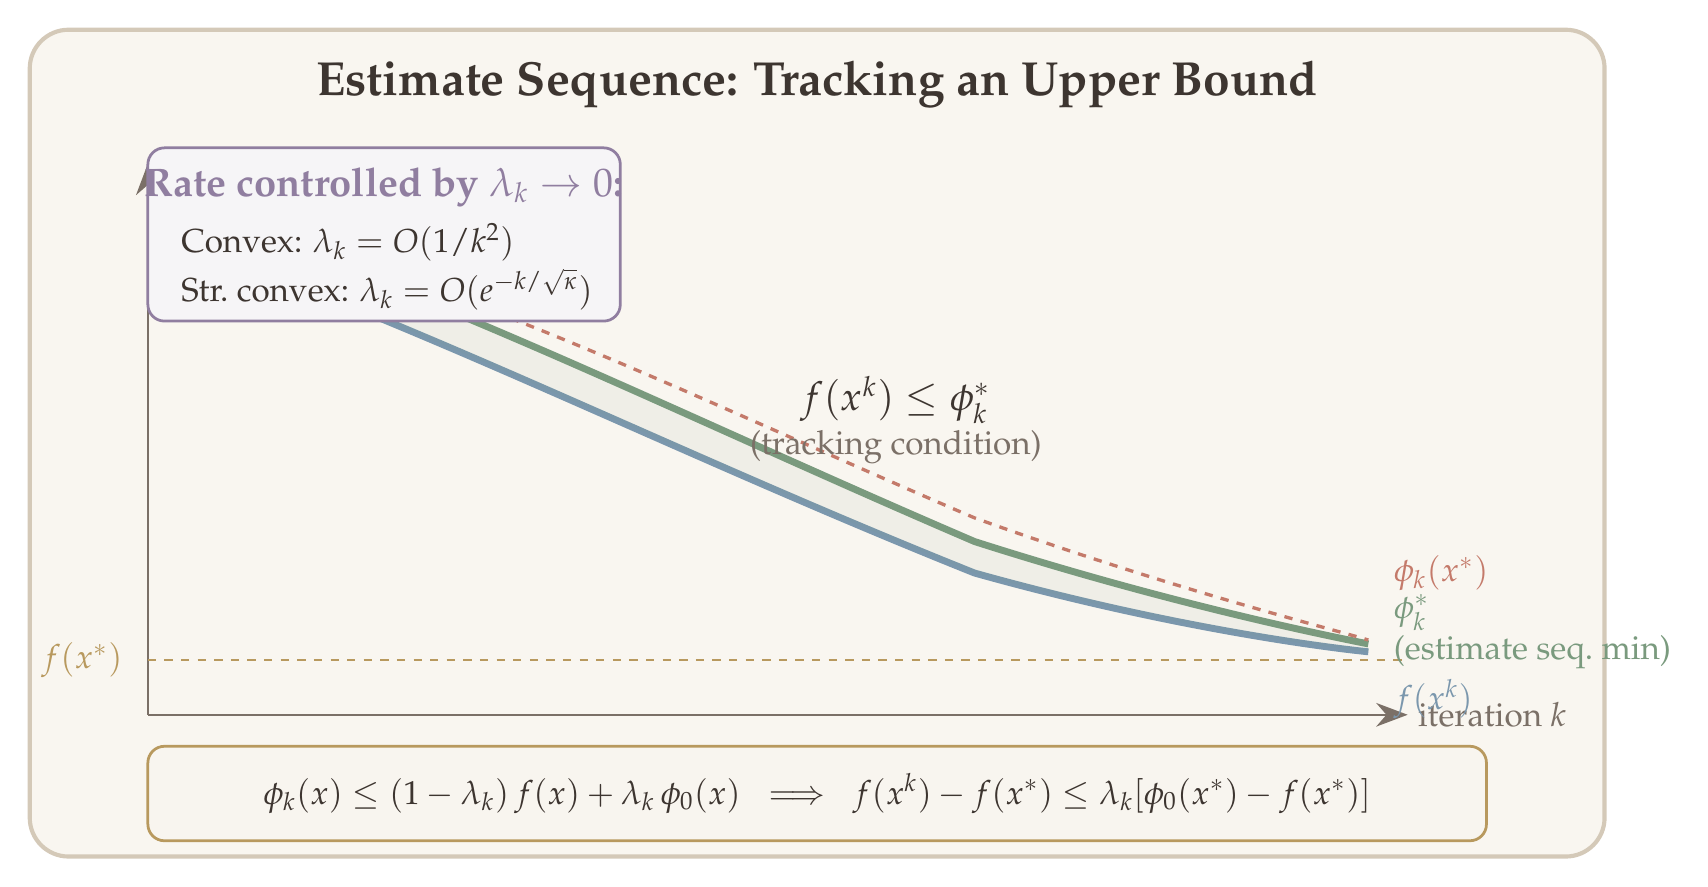
\begin{tikzpicture}[
  >={Stealth[length=4mm, width=3mm]},
  every node/.style={text=dkbrown, font=\large},
]

% Background
\fill[cream, rounded corners=14pt] (0,0) rectangle (20,10.5);
\draw[border, line width=1.5pt, rounded corners=14pt] (0,0) rectangle (20,10.5);

% Title
\node[font=\LARGE\bfseries, text=dkbrown] at (10,9.8) {Estimate Sequence: Tracking an Upper Bound};

% Axes
\draw[wmgray, line width=0.8pt, ->] (1.5,1.8) -- (17.5,1.8)
  node[right, font=\large, text=wmgray] {iteration $k$};
\draw[wmgray, line width=0.8pt, ->] (1.5,1.8) -- (1.5,8.8);

% f(x*) baseline
\draw[rwgold, line width=0.8pt, dashed] (1.5,2.5) -- (17.5,2.5);
\node[font=\large, text=rwgold, anchor=east] at (1.3,2.5) {$f(x^*)$};

% phi_0 label
\node[font=\large, anchor=west] at (1.8,8.5) {$\phi_0(x) = f(x^0) + \tfrac{\gamma_0}{2}\|x - x^0\|^2$};

% phi_k^* curve (estimate sequence minimum) — decreasing
\draw[sage, line width=2.5pt]
  (2.5,8.0) .. controls (5.5,7.0) and (8.5,5.5) .. (12,4.0)
  .. controls (14.5,3.2) and (16.5,2.8) .. (17.0,2.7);
\node[font=\large, text=sage, anchor=west] at (17.2,3.1) {$\phi_k^*$};
\node[font=\large, text=sage, anchor=west] at (17.2,2.6) {(estimate seq.\ min)};

% f(x^k) curve (below phi_k^*)
\draw[stblue, line width=2.5pt]
  (2.5,7.6) .. controls (5.5,6.5) and (8.5,5.0) .. (12,3.6)
  .. controls (14.5,2.9) and (16.5,2.65) .. (17.0,2.6);
\node[font=\large, text=stblue, anchor=west] at (17.2,2.0) {$f(x^k)$};

% Shaded region between the curves
\fill[sage, opacity=0.08]
  (2.5,7.6) .. controls (5.5,6.5) and (8.5,5.0) .. (12,3.6)
  .. controls (14.5,2.9) and (16.5,2.65) .. (17.0,2.6)
  -- (17.0,2.7) .. controls (16.5,2.8) and (14.5,3.2) .. (12,4.0)
  .. controls (8.5,5.5) and (5.5,7.0) .. (2.5,8.0) -- cycle;

% phi_k(x*) curve (dashed, above phi_k^*)
\draw[terracotta, line width=1.2pt, dashed]
  (2.5,8.0) .. controls (5.5,7.3) and (8.5,5.8) .. (12,4.3)
  .. controls (14.5,3.4) and (16.5,2.9) .. (17.0,2.75);
\node[font=\large, text=terracotta, anchor=west] at (17.2,3.6) {$\phi_k(x^*)$};

% Key relationship label
\node[font=\Large\bfseries] at (11.0,5.8) {$f(x^k) \leq \phi_k^*$};
\node[font=\large, text=wmgray] at (11.0,5.2) {(tracking condition)};

% lambda_k annotation box
\draw[lavender, line width=1pt, rounded corners=6pt, fill=lavender!8]
  (1.5,6.8) rectangle (7.5,9.0);
\node[font=\Large\bfseries, text=lavender] at (4.5,8.5) {Rate controlled by $\lambda_k \to 0$:};
\node[font=\large, anchor=west] at (1.8,7.8) {Convex: $\lambda_k = O(1/k^2)$};
\node[font=\large, anchor=west] at (1.8,7.2) {Str.\ convex: $\lambda_k = O(e^{-k/\sqrt{\kappa}})$};

% Bottom annotation box
\draw[rwgold, line width=1pt, rounded corners=6pt, fill=rwgold!10]
  (1.5,0.2) rectangle (18.5,1.4);
\node[font=\large] at (10.0,0.8) {%
  $\phi_k(x) \leq (1-\lambda_k)\,f(x) + \lambda_k\,\phi_0(x)
  \;\;\Longrightarrow\;\;
  f(x^k) - f(x^*) \leq \lambda_k[\phi_0(x^*) - f(x^*)]$};

\end{tikzpicture}
\end{document}
